%! TEX root = ./main.tex

\section{Technical preliminaries}
\label{sec:notations formal result}



In this section, we present preparatory material on $\beta$-expansions, and we split the proof of Theorem \ref{thm:informal equivalence kolmogorov complexity computable} in subcases dealt with in the remaining sections of the paper.
% \subsection{beta-expansions}
\subsection{\texorpdfstring{$\beta$-expansions}{-expansions} and dynamical maps}
\noindent Let $\beta \in (1,2]$. Following \cite{parry1960beta}, we say that $\xf \in \{0,1\}^\omega$ is a $\beta$-expansion of 
$s \in I_\beta := \ibet$ if
\begin{equation}\label{eq:definition beta expansion}
	s = \delta_\beta(\xf),
\end{equation}
where 
\begin{equation}\label{eq:definition of delta beta}
	\begin{array}{lccl}
		\delta_\beta : & \{0,1\}^\omega & \to & I_\beta\\
		& \xf & \mapsto & \displaystyle \sum_{i=1}^{\infty} \xf_i \beta^{-i}.
	\end{array}
\end{equation}
To see that $\delta_\beta$ indeed maps to $I_\beta$, note that $\delta_\beta(0^\infty) = 0$ and $\delta_\beta(1^\infty) = \frac{1}{\beta-1}$. For $x \in \{0,1\}^\ast$, we use the shorthand $\delta_\beta(x):= \sum_{i=1}^{|x|}x_i\beta^{-i}$ instead of the more cumbersome $\delta_\beta(x0^\infty)$. As already mentioned in Section \ref{sec:introduction}, there are, in general, multiple sequences $\xf \in \{0,1\}^\omega$ generating a given $s$ according to (\ref{eq:definition beta expansion}); we denote by $\Sigma_\beta(s) := \delta_\beta^{-1}(\{s\})$ the set of all $\beta$-expansions of $s \in I_\beta$. For instance, as explained in Section \ref{sec:introduction}, for $G = \frac{1 + \sqrt{5}}{2}$ we have $\Card{\Sigma_G(1)} = \infty$. Moreover, for each $\beta \in (1,G)$, the set of $\beta$-expansions for each $s \in I_\beta$ is uncountable, i.e., $\Card{\Sigma_\beta(s)} = 2^{\aleph_0}$ \cite[Theorem 3]{erdos1990characterization}. 

For $s \in I_\beta$, we define the greedy $\beta$-expansion $\gf_\beta(s)$ to be the lexicographically maximal element of $\Sigma_\beta(s)$. As mentioned in Section \ref{sec:introduction}, Algorithm \ref{alg:greedy algorithm beta expansion} computes $\gf_\beta(s)$. We now show that this algorithm can be interpreted as a dynamical system. This interpretation will be crucial to the proof of Theorem \ref{thm:informal equivalence kolmogorov complexity computable}. Inspection of Algorithm \ref{alg:greedy algorithm beta expansion} reveals that the variable ``$r$'' realizes the greedy map $G_\beta : I_\beta \to I_\beta$ \cite[Section 1, p.2]{baker2015induced}:
\begin{equation}\label{eq:greedy map}
	G_\beta (r) = \begin{cases}
		\beta r, \ \ \text{if} \ r < \frac{1}{\beta},\\
		\beta r - 1, \ \ \text{if} \ r \geq \frac{1}{\beta}, 
	\end{cases} \ \ \forall r \in I_\beta.
\end{equation}
Further, the variable ``$b$'' in Algorithm \ref{alg:greedy algorithm beta expansion} realizes the following function
\begin{equation}
	d_{\beta}  (r) = \begin{cases}
		0, \ \ \text{if} \ r < \frac{1}{\beta},\\
		1, \ \ \text{if} \ r \geq \frac{1}{\beta}, 
	\end{cases} \ \ \forall r \in I_\beta,
\end{equation}
that generates one bit of the greedy $\beta$-expansion of $r$. Note that $G_\beta(r) = \beta r - d_\beta(r)$, for $r \in I_\beta$. Finally, the greedy $\beta$-expansion is shown to be given by
\begin{equation}\label{eq:greedy beta exp as digit + iterative map}
	\gf_\beta(s) = \coprod_{i=0}^\infty d_{\beta}\left(G_\beta^{i}(s)\right).
\end{equation}
Remark that $G_\beta$ can be interpreted as a bit-shifting and a bit-extraction device. Let $s \in [0,1]$ and denote its greedy $\beta$-expansion by $\xf$. Then, one has 
\begin{equation}
	G_\beta(s) = \beta s - d_\beta(s) = \beta \sum_{i=1}^\infty \xf_i \beta^{-i} - d_\beta(s) = \xf_1 + \sum_{i=2}^\infty \xf_i \beta^{-i+1} - \xf_1 = \sum_{i=1}^\infty \xf_{i+1} \beta^{-i},
\end{equation}
which shows that application of $G_\beta$ simply shifts the sequence $\xf$ by one position to the left. It now follows directly that iterating $G_\beta$ $n$ times effects a left-shift by $n$ positions according to 
\begin{equation}\label{eq:n iterations of greedy map is same as shifting n bits}
	G^n_\beta(s) = \sum_{i=1}^\infty \xf_{i+n} \beta^{-i}.
\end{equation}
Moreover, we can also interpret the greedy map as a bit-extraction device, namely by noting that
\begin{equation}\label{eq:n iterations of greedy map is same as reading the first n bits}
	s - \frac{1}{\beta^n} G^n_\beta(s) = \sum_{i=1}^\infty \xf_i \beta^{-i} - \frac{1}{\beta^n}\sum_{i=1}^\infty \xf_{i+n} \beta^{-i} = \sum_{i=1}^n\xf_i \beta^{-i} = \delta_\beta(\xf_{1: n}).
\end{equation}
We now note that the generation the successive prefixes of the greedy $\beta$-expansion can be cast into the following equation $(E_\Theta)$, depending on the parameter $\Theta = (\beta,R_0) \in (1,2) \times I_\beta$, that describes an iterative process $R_1,R_2,\ldots$, by
\begin{equation}\label{eq:greedy map as system of equations}
		R_{i+1} = \displaystyle G_\beta(R_i),
	\tag{$E_\Theta$}
\end{equation}
for $i \in \N_0$. Setting $R_0 = s \in I_\beta$, we recover
\begin{equation}\label{eq:greedy expansion from evolution of R i}
	\gf_\beta(s) \overset{(\ref{eq:greedy beta exp as digit + iterative map})}{=} \coprod_{i=0}^\infty d_{\beta}\left(R_i\right),
\end{equation}
hence the greedy $\beta$-expansion of $s$ is deduced from the variable $R_i$. The successive values taken by $R_i$ correspond to the evolution of a discrete dynamical system with no inputs. We can further transform the generation of the greedy $\beta$-expansion into a discrete dynamical system with one parameter $\beta \in (1,2)$, always starting on $R_0 = 0$, and presented with an input $\ssf = s_0s_1\ldots \in I_\beta^\omega$, as follows. 
\begin{equation}\label{eq:greedy map as dynamical system}
	\begin{array}{rl}
		R_{i+1} &= \displaystyle G_\beta(R_i + s_i),
	\end{array}
	\tag{$E_{\beta}$}
\end{equation}
for $i \in \N_0$, with $R_0 = 0$. When presented with input $\ssf = s_0s_1 \in I_\beta^\omega$, $E_\beta$ is seen as a mapping $I_\beta^\ast \to \{0,1\}^\ast$ by $E_\beta(\epsilon) := \epsilon$ and
\begin{equation}\label{eq:inferring prefix of greedy expansion from R i E beta}
	E_\beta(s_0s_1\ldots s_{n-1}) := \coprod_{i=0}^{n-1} d_\beta(R_i + s_i), 
\end{equation}
for all $n \in \N$, and as a mapping $ I_\beta^\omega \to \{0,1\}^\omega$ through
\begin{equation}\label{eq:inferring greedy expansion from R i E beta}
	E_\beta(\ssf) := \coprod_{i=0}^{\infty} d_\beta(R_i + s_i).
\end{equation}

Note that by setting $s_0 = s \in I_\beta$ and $s_i = 0$ for $i \in \N$, $E_\beta(\ssf) = \gf_\beta(s)$. Finally, note that we can adapt (\ref{eq:greedy map as dynamical system}) so that it generates the greedy $\beta$-expansion by chunks. Let $N \in \N$, and consider 
\begin{equation}\label{eq:greedy map chunks as dynamical system} \tag{\text{$E^N_\beta$}}
	R_{i+1} = G_\beta^N(R_i + s_i).
\end{equation}
We also generalize the function $d_\beta$ to $d_\beta^N$ that generates $N$ bits of greedy $\beta$-expansion as
\begin{equation}\label{eq:definition multiple digit map}
	d_\beta^N(r) := \coprod_{i=0}^{N-1} d_{\beta}\left(G_\beta^{i}(s)\right) \overset{(\ref{eq:greedy expansion from evolution of R i})}{=} \gf_\beta(r)_{1:N}, \ \text{for} \ r \in I_\beta.
\end{equation}
Note that indeed, $d_\beta^1 = d_\beta$. When presented with input $\ssf = s_0s_1 \in  I_\beta^\omega$, we can see $E^N_\beta$ as a mapping $ I_\beta^\ast \to \{0,1\}^\ast$ by $E^N_\beta(\epsilon) := \epsilon$ and
\begin{equation}\label{eq:inferring prefix of chunks of greedy expansion from R i E beta}
	E^N_\beta(s_0s_1\ldots s_{n-1}) := \coprod_{i=0}^{n-1} d^N_\beta(R_i + s_i), 
\end{equation}
for all $n \in \N$, and as a mapping $I_\beta^\omega \to \{0,1\}^\omega$ through
\begin{equation}\label{eq:inferring chunks of greedy expansion from R i E beta}
	E^N_\beta(\ssf) := \coprod_{i=0}^{\infty} d^N_\beta(R_i + s_i).
\end{equation}
Again, setting $s_0 = s \in I_\beta$ and $s_i = 0$ for $i \in \N$ yields $E^N_\beta(\ssf) = \gf_\beta(s)$. Similar considerations apply to the lazy $\beta$-expansion, but we do not detail it as this is not needed for our proofs.
% One can also define the lazy $\ellf_\beta := \inf_L\left(\Sigma_\beta(s)\right)$. 
% Following \cite[Section 2]{dajani2002greedy} 
% the lazy $\beta${-expansion} can be generated as follows. Analogously to the greedy map $G_\beta$ above, we define the lazy map according to
%  $L_\beta : I_\beta \to I_\beta$ \cite[Section 1]{baker2015induced}:
% \begin{equation}
% 	L_\beta (r) = \begin{cases}
% 		\beta r, \ \ \text{if} \ r \leq \frac{1}{\beta(\beta-1)},\\
% 		\beta r - 1, \ \ \text{if} \ r > \frac{1}{\beta(\beta-1)}, 
% 	\end{cases} \ \ \forall r \in I_\beta.
% \end{equation}
% The bits of the lazy $\beta$-expansion are then computed by the following function
% \begin{equation}
% 	d_{\beta,lazy}  (r) = \begin{cases}
% 		0, \ \ \text{if} \ r \leq \frac{1}{\beta(\beta-1)},\\
% 		1, \ \ \text{if} \ r > \frac{1}{\beta(\beta-1)}, 
% 	\end{cases} \ \ \forall r \in I_\beta.
% \end{equation}
% Finally, the lazy $\beta$-expansion is shown to be given by
% \begin{equation}
% 	\ellf_\beta(s) = \coprod_{i=0}^\infty d_{\beta,lazy}\left(L_\beta^{i}(s)\right).
% \end{equation}



% \subsection{Algorithmic complexity}

% \subsection{Kolmogorov complexity of beta-expansions}
% \label{subsec:Kolmgorov complexity}


% We now proceed in establishing solid ground for the study of algorithmic complexity. Recall the notion of universal effective algorithm introduced in previous section. Following \cite[Definition 3.4]{calude2002information}\cite[Chapter 14.2]{cover1999elements}\cite[Definition 2.1.1]{li2008introduction}, the  algorithmic complexity of a binary sequence $x \in \{0,1\}^\ast$ with respect to a given universal effective algorithm $U : \{0,1\}^\ast \to \{0,1\}^\ast$ is
% \begin{equation}\label{eq:informal definition relative Kolmorogov complexity}
% 	K_U[x] := \min \{ \len u : u \in \{0,1\}^\ast, U(u) = x\}.
% \end{equation}
% Following \cite[Definition 3.4]{calude2002information}, we say that $x^\ast$ is the canonical program for $x$ with respect to $U$ if 
% \begin{equation}
% 	x^\ast := \min \left\{ u \in \{0,1\}^\ast : U(u) = x \right\},
% \end{equation}
% where the $\min$ is taken with respect to the quasi-lexicographical order. Note that $|x^\ast| = K_U[x]$.


%Definition (\ref{eq:informal definition relative Kolmorogov complexity}) is usually referred to as conditional algorithmic complexity, see \cite[Chapter 14.2]{cover1999elements}, where the qualifier ``conditional'' indicates knowledge of $|x|$. 

% Following \cite[Theorem 14.2.1]{cover1999elements}, we now show that the choice of $U$ is somewhat not important. 
% \begin{lemma}
% 	Let $V : \{0,1\}^\ast \to \{0,1\}^\ast$ be another universal effective algorithm. Then, there exists $c > 0$ such that for all $x \in \{0,1\}^\ast$,
% 	\begin{equation}
% 		\left| K_U[x] - K_V[x]\right| \leq c.
% 	\end{equation}
% \end{lemma}
% \begin{proof}
% 	As $U$ is a universal effective algorithm, there exists $p \in \{0,1\}^\ast$ such that 
% 	\begin{equation}
% 		U(\langle p, x \rangle) = V(x), \text{ for all } x \in \{0,1\}^\ast. 
% 	\end{equation}
% Let $x \in \{0,1\}^\ast$, and let $x^\ast \in \{0,1\}^\ast$ be the canonical program for $x$ with respect to $V$. Then, $U(\langle p, x^\ast\rangle) = V(x^\ast) = x$. It follows that $K_U[x] \leq |\langle p, x^\ast \rangle| \leq 2|p| + |x^\ast| + 1 = 2|p|+ 1+ K_V[x]$. We let $c_1 := 2|p| + 1$, and then $K_U[x] \leq K_V[x] + c_1$. Likewise, we can show that there is a constant $c_2 > 0$ such that $K_V[x] \leq K_U[x] + c_2$. The lemma follows by letting $c = \max(c_1,c_2)$.
% \end{proof}
% Then, the definition of algorithmic complexity relatively to a specific universal effective algorithm is invariant up to a positive additive constant. From now on, we fix a universal effective algorithm $\Uref$, and define the (absolute) algorithmic complexity of the binary sequences $x$ as
% \begin{equation}\label{eq:informal definition absolute Kolmorogov complexity}
% 	\begin{array}{lccl}
% 		K[\cdot] : & \{0,1\}^\ast & \to & \N\\ 
% 			& x &	\mapsto & K_{\Uref}[x].
% 	\end{array}
% \end{equation}

% In this paper, we are interested in comparing the algorithmic complexity of binary expansions and $\beta$-expansions. As the expansions are of infinite length and algorithmic complexity is defined for finite binary sequences only, we need an adequate extension of algorithmic complexity to infinitely long sequences. Specifically, following \cite[Definition 10.9]{balcazar2012structural}, we shall consider the algorithmic complexity of $n$-prefixes $\xf_{1: n}$ of such an infinite sequence $\xf$. For simplicity of notations, we shall write
% \begin{equation}
% 	K[\xf|n] := K[\xf_{1: n}], \ \text{ for all } \xf \in \{0,1\}^\omega, \ \text{ and all } n \in \N.
% \end{equation}
% The above definition allows to study the algorithmic complexity of $\beta$-expansions.



\subsection{\texorpdfstring{Algorithmic complexity of binary expansions}{}}

We are now ready to commence our investigation of the algorithmic complexity of $\beta$-expansions, specifically with an eye towards comparison with the behavior of the algorithmic complexity of binary expansions. 

% First, recall that binary expansions are essentially unique, concretely unique up to the 2-ambiguity property discussed in Section \ref{sec:introduction}. On the other hand, $\beta$-expansions are highly non-unique as exemplified in Section \ref{sec:introduction}. The goal of our analysis is to develop an understanding of how this nonuniqueness is reflected in terms of algorithmic complexity. 

We formalize the following statement from \cite[Section IV]{balcazar1997hierarchy}: ``In the cases where $\delta_2$ is not injective, [...]\hspace{0.5mm}the two inverse images [...]\hspace{0.5mm}have essentially (up to a small additive term) the same Kolmogorov complexity''. To our knowledge, the latter assertion is not made formal in the literature. This result allows to make a first simplification to the proof of Theorem \ref{thm:informal equivalence kolmogorov complexity computable}: the variable $\xf$ in (\ref{eq:equivalence kolmogorov complexity binary beta expansions}) can be chosen to be the greedy binary expansion, instead of working with either the greedy or the lazy expansion.
\begin{lemma}\label{lem:greedy and lazy expansion have same K complexity}
	There exists $c > 0$ such that, for every $s \in [0,1]$, the greedy binary expansion $\gf_2(s)$ and the lazy binary expansion $\ellf_2(s)$ satisfy 
\begin{equation}\label{eq:greedy and lazy binary expansions have same algorithmic complexity}
	\left|K[\gf_2(s)|n] - K[\ellf_2(s)|n]\right| \leq c, \ \forall n \in \N.
\end{equation}
\end{lemma}
\begin{proof}
As explained in Section \ref{sec:introduction}, the greedy and lazy binary expansion of a given real number $s \in [0,1]$ differ only when the greedy expansion ends with $0^\infty$; in this case, the lazy expansion ends with $1^\infty$. Such numbers $s$ are said to be ``dyadic''; the set of all dyadic numbers is denoted by $\D$. Now, for $s \notin \D$, one has $\ellf_2(s) = \gf_2(s)$ so that (\ref{eq:greedy and lazy binary expansions have same algorithmic complexity}) holds trivially. When $s \in \D$, the operations underlying (\ref{eq:greedy expansion ending with infinitetail of zeros})-(\ref{eq:lazy expansion ending with infinitetail of ones}), can be cast into an effective algorithm $\varphi$ summarized in Algorithm \ref{alg:generator of greedy expansion fixed input}, such that $\varphi(\gf_2(s)_{1: n}) = \ellf_2(s)_{1: n}$, for all $n \in \N$.
\begin{algorithm}
	\caption{Conversion from a greedy prefix to a lazy prefix}\label{alg:generator of greedy expansion fixed input}
	\begin{algorithmic}[1]
		\Require  $x \in \{0,1\}^\ast$
		\State Find the position $n$ of the last $1$ in $x$ 
		\State $x_n \gets 0$
		\For{$i = n+1, \ldots, |x|$}
		\State $x_i \gets 1$
		\EndFor
		\State \Return $x$
	\end{algorithmic}
	\end{algorithm}

Note that $\varphi$ essentially finds the last bit equal to $1$ of its input $x \in \{0,1\}^\ast$, switches it to $0$, and then switches all the following bits to $1$. Conversely, one can devise an effective algorithm $\psi$ that finds the last $0$ of its input $x \in \{0,1\}^\ast$, switches it to $1$, and then switches all the following bits to $0$. This last algorithm converts a lazy expansion into a greedy expansion, i.e. $\psi(\ellf_2(s)_{1: n}) = \gf_2(s)_{1: n}$ for all $s \in [0,1]$ and all $n \in \N$. By application of Lemma \ref{lem:if two sequences are connected through an algorithm, they have same kolmogorov complexity}, there exists two constants $c_\varphi,c_\psi > 0$ such that
\begin{equation}
	\begin{array}{l}
	K[\ellf_2(s) | n] \leq K[\gf_2(s)|n] + c_\varphi,\\
	K[\gf_2(s)|n] \leq K[\ellf_2(s)|n] + c_\psi,
	\end{array} \ \forall n \in \N, \ \text{and} \ \forall s \in \D.
\end{equation}
Setting $c := \max(c_\varphi, c_\psi)$ finishes the proof.
\end{proof}

Thanks to Lemma \ref{lem:greedy and lazy expansion have same K complexity}, Theorem \ref{thm:informal equivalence kolmogorov complexity computable} can be restated as follows. For all $s \in [0,1]$ and all computable $\beta \in (1,2]$, there exist $\xf \in \Sigma_\beta(s)$ and $c > 0$ such that
\begin{equation}\label{eq:equivalence algorithmic complexity beta expansion binary expansion}
	\left|K[\xf|n] - K[\gf_2(s)|\lceil n \log_2(\beta)\rceil] \right| \leq c, \ \ \forall n \in \N.
\end{equation}
This result constitutes a vast extension of \cite[Theorem 3]{staiger2002kolmogorov}, which establishes an equivalent fact for $q$-ary expansions, where $q \in \N_2$.

\subsection{\texorpdfstring{Related work on $q$-ary expansions}{}}

Fix $q \in \N_2$. A $q$-ary expansion of a given $s \in [0,1]$ is an infinite $q$-ary sequence $\xf \in A_q^\omega$ satisfying
\begin{equation}
	s = \sum_{i=1}^\infty \xf_i q^{-i} =: \delta_q(\xf).
\end{equation}
For $x \in A_q^\ast$, we use the shorthand $\delta_q(x)$ to denote $\delta_q(x0^\infty)$. It was shown in \cite[Section 7.2]{calude2002information} that $q$-ary expansions also exhibit a $2$-ambiguity property; specifically for $\delta_q(\xf)$ irrational, $\delta_q(\xf) = \delta_q(\xf')$ implies $\xf = \xf'$, whereas for rational $\delta_q(\xf)$, there can be two different $q$-ary sequences that generate it. We define the greedy $q$-ary expansion $\gf_q(s)$ of a given $s \in [0,1]$ to be the lexicographically larger $q$-ary expansion of $s$. 

We first extend the notion of algorithmic complexity to $q$-ary sequences. Note that as each $b \in A_q$ can be encoded with a binary sequence of length $\lceil \log_2(q) \rceil$, then each $x \in A_q^\ast$ can be encoded by a binary sequence of length $|x| \lceil \log_2(q) \rceil$, that we denote $x^{(2)}$. For $x \in A_q^\ast$, we set $K[x] := K[x^{(2)}]$, and for $\xf \in A_q^\omega$, we let $K[\xf|n] := K[(\xf_{1:n})^{(2)}]$. 
\begin{theorem}\cite[Theorem 3]{staiger2002kolmogorov}\label{thm:staiger invariance}
	For all $q \in \N_2$ and  all $s \in [0,1]$, there exists $c > 0$ such that
\begin{equation}\label{eq:equivalence Kolmogorov complexity q ary expansions}
	\left| K\left[\gf_q(s)|n\right] - K\left[\gf_2(s)|\lceil n\log_2(q) \rceil\right]\right| \leq c, \ \ \text{for all} \ n \in \N, \ s \in [0,1].
\end{equation}
\end{theorem}
\begin{proof} We present the proof of the inequality
\begin{equation}
	 K\left[\gf_q(s)|n\right] \leq K\left[\gf_2(s)|\lceil n\log_2(q) \rceil\right] + c, \ \ \text{for all} \ n \in \N, \ s \in [0,1],
\end{equation}
and the converse inequality is analogously proven. The above inequality will be proved by showing that there exists an effective algorithm $\varphi : \{0,1\}^\ast \to \{0,1\}^\ast$ and $b_n \in \{0,1\}$, such that 
\begin{equation}
	\varphi(b_n \, \gf_2(s)_{1:\lceil n\log_2(q) \rceil}) = \gf_q(s)_{1:n}, \ \text{for all} \ n \in \N.
\end{equation} 
We make three observations, that allow to construct $\varphi$.
\begin{enumerate}[label = (\alph*)]
	\item \label{item:observation spacings between finite expansions} For $n \in \N$, let $S_n(q) := \{ \delta_q(x) : x \in A_q^n\}$. Then, for all $n \in \N$, $S_n(q) = \{ m q^{-n} : m \in \{0, \ldots, q^n - 1\}\}$, and $\delta_q$ is bijective from $A_q^n$ to $S_n(q)$. Below we displayed $S_n(q)$ for $n = 3$ and $q = 3$.
	\begin{figure}[H]
		\centering
		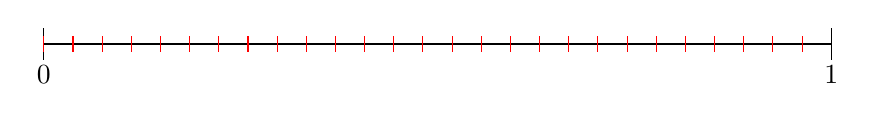
\begin{tikzpicture}[scale = 10]
			\draw (0,0) -- (1,0);
			\draw (0,0) -- (1,0);
			\draw (0,-0.02) -- (0,0.02);
			\draw (1,-0.02) -- (1,0.02);
			\node[below] at (0,-0.015){$0$};
			\node[below] at (1,-0.015){$1$};
			\foreach \x in {0, ..., 26}
			{\draw[red] (\x/27,-0.01) -- (\x/27,0.01);}
		\end{tikzpicture}
		\caption{Each red line corresponds to one element $t$ in $S_3$, which in turn corresponds to exactly one element $x$ in $A_3^3$, being the preimage of $t$ by $\delta_3$.}
		\label{fig:spacings between finite q ary expansions}
	\end{figure}
		This observation essentially says that $S_n(q)$ is made of elements that are isolated and $q^{-n}$ apart. The 2-ambiguity of $q$-ary expansions crucially relies on this property.
	\item \label{item:observation greedy prefix is the immediate predecessor}For $s \in [0,1]$, $n \in \N$, $g_q(s)_{1:n}$ is exactly the preimage by $\delta_q$ of the number $t \in S_n$ that is the immediate predecessor of $s$. Below we displayed this number $t$ for $n = 3$, $q = 3$ and $s = 0.745$.
	\begin{figure}[H]
		\centering
		\begin{tikzpicture}[scale = 10]
			\draw (0,0) -- (1,0);
			\draw (0,0) -- (1,0);
			\draw (0,-0.02) -- (0,0.02);
			\draw (1,-0.02) -- (1,0.02);
			\draw[blue] (0.745,-0.02) -- (0.745,0.02);
			\node[below] at (0,-0.015){$0$};
			\node[below] at (1,-0.015){$1$};
			\node[below] at (0.745,-0.015){$s$};
			\draw[->] (0.73,0.03) -- (0.74,0.012);
			\node[above] at (0.73,0.025){$t$};
			\foreach \x in {0, ..., 26}
			{\draw[red] (\x/27,-0.01) -- (\x/27,0.01);}
		\end{tikzpicture}
		\caption{Here $t = \delta_3(\gf_3(s)_{1:3})$.}
	\end{figure}
	\item \label{item:observation binaru exp is close to the real number}Let $m \in \N$, and $x \in \{0,1\}^m$. $x$ can be the $m$-prefix of the greedy binary expansion of any number in $[\delta_2(x), \delta_2(x) + 2^{-m})$.
	\begin{figure}[H]
		\centering
		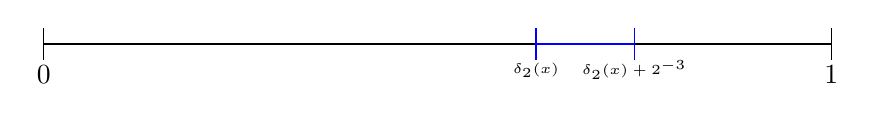
\begin{tikzpicture}[scale = 10]
			\draw (0,0) -- (1,0);
			\draw (0,0) -- (1,0);
			\draw (0,-0.02) -- (0,0.02);
			\draw (1,-0.02) -- (1,0.02);
			\draw[blue] (0.625,-0.02) -- (0.625,0.02);
			\draw[blue] (0.75,-0.02) -- (0.75,0.02);
			\draw[blue, thick] (0.625,0) -- (0.75,0);
			\node[below] at (0,-0.015){$0$};
			\node[below] at (1,-0.015){$1$};
			\node[below] at (0.625,-0.012){\tiny $\delta_2(x)$};
			\node[below] at (0.75,-0.008){\tiny $\delta_2(x) + 2^{-3}$};
		\end{tikzpicture}
		\caption{Here we displayed the range of real numbers that admit $x = 0.101$ as prefix of their greedy binary expansion.}
	\end{figure}
\end{enumerate}
By combining the above three observations, we deduce that for $n,m \in \N$, and $x \in \{0,1\}^m$, there are less than $\lceil 2^{-m}/q^{-n} \rceil + 1$ elements in $A_q^n$ that correspond to the $n$-prefix of the greedy $q$-ary expansion of one of the real numbers whose greedy binary expansion starts with $x$.  The set of $n$-prefixes of greedy $q$-ary expansions associated with $x$ is denoted $A_q^n(x)$. Below, we displayed this result for $n = m = 3$ and $x = 0.101$.
\begin{figure}[H]
	\centering
	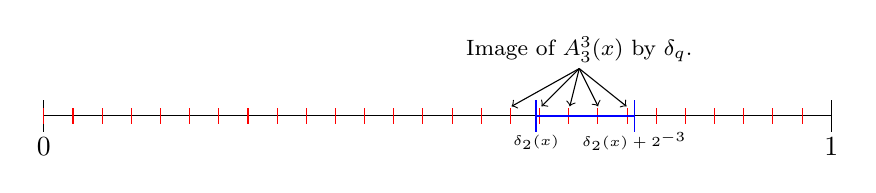
\begin{tikzpicture}[scale = 10]
		\draw (0,0) -- (1,0);
		\draw (0,0) -- (1,0);
		\draw (0,-0.02) -- (0,0.02);
		\draw (1,-0.02) -- (1,0.02);
		\node[below] at (0,-0.015){$0$};
		\node[below] at (1,-0.015){$1$};
		\foreach \x in {0, ..., 26}
		{\draw[red] (\x/27,-0.01) -- (\x/27,0.01);}
		\draw[blue] (0.625,-0.02) -- (0.625,0.02);
		\draw[blue] (0.75,-0.02) -- (0.75,0.02);
		\draw[blue, thick] (0.625,0) -- (0.75,0);
		\draw[->] (0.68,0.06) -- (0.74,0.012);
		\draw[->] (0.68,0.06) -- (0.704,0.012);
		\draw[->] (0.68,0.06) -- (0.668,0.012);
		\draw[->] (0.68,0.06) -- (0.632,0.012);
		\draw[->] (0.68,0.06) -- (0.594,0.012);
		\node[above] at (0.68,0.055){\footnotesize Image of $A_3^3(x)$ by $\delta_q$.};
		\node[below] at (0.625,-0.012){\tiny $\delta_2(x)$};
		\node[below] at (0.75,-0.008){\tiny $\delta_2(x) + 2^{-3}$};
	\end{tikzpicture}
	\caption{In blue, we represented the set $I(x)$ of real numbers for which $x$ is a prefix of their greedy binary expansion. In red are all the numbers that are the image of elements of $A_3^3$ through $\delta_3$. The red elements designated by an arrow are elements in $A_3^3$ that are a prefix of the greedy ternary expansion of at least one real number in $I(x)$. We observe that there are 5 such elements, which is in accordance with the above formula $\lceil 2^{-3}/3^{-3} \rceil + 1 = 5$.}
\end{figure}

Now, let $s \in [0,1]$ and $n,m \in \N$. By the above discussion, $\gf_q(s)_{1:n} \in A_q^n(\gf_2(s)_{1:m})$. Therefore, one just needs $\gf_2(s)_{1:m}$ and the position $b_n \in \{0, \ldots, \lceil 2^{-m}/q^{-n} \rceil \}$ of $\gf_q(s)_{1:n}$ in the lexicographical enumeration of $A_q^n(\gf_2(s)_{1:m})$ to deduce $\gf_q(s)_{1:n}$. Remark that in the particular case $m = \lceil n \log_2(q)\rceil$, we have $b_n \in \{0, 1\}$. This concludes the construction the algorithm $\varphi$, as we have derived a method to deduce $\gf_q(s)_{1:n}$ from $b_n \, \gf_2(s)_{1:\lceil n \log_2(q)\rceil}$, for all $n \in \N$ and all $s \in [0,1]$.

Now, from Lemma \ref{lem:if two sequences are connected through an algorithm, they have same kolmogorov complexity}, there exists $C > 0$ such that
\begin{equation}\label{eq:g q g 2 and binary pos}
	K[\gf_q(s)_{1:n}] \leq K[b_n \, \gf_2(s)_{1:\lceil n \log_2(q)\rceil}] + C.
\end{equation}
Now, this is easy to conceive two effective algorithms $\varphi_0$ and $\varphi_1$ such that $\varphi_0(x) = 0x$ and $\varphi_1(x) = 1x$, for all $x \in \{0,1\}$, and hence by Lemma \ref{lem:if two sequences are connected through an algorithm, they have same kolmogorov complexity}, there exists $c_0,c_1$ such that 
\begin{equation}
	K[0x] \leq x + c_0, \ \text{and} \ K[1x] \leq x + c_1, \ \text{for all} \ x \in \{0,1\}^\ast.
\end{equation}
Injecting in (\ref{eq:g q g 2 and binary pos}) gives
\begin{align}%\label{eq:g q g 2 and binary pos 2}
	K[\gf_q(s)_{1:n}] &\leq K[\gf_2(s)_{1:\lceil n \log_2(q)\rceil}] + C + c_{b_n}\\
	&\leq K[\gf_2(s)_{1:\lceil n \log_2(q)\rceil}] + C + \max \{c_0, c_1\}.
\end{align}
Setting $c := C + \max \{c_0, c_1\}$ finishes the proof.
\end{proof}

% The proof relies on the following critical observation, which is a premisse to the 2-ambiguity property of $q$-ary expansion.

% \begin{proof}
% Suppose we know the first $\lceil n \log_2(q) \rceil$ bits of $\gf_2(s)$. Note that 
% \begin{equation}
% 	0 \leq s - \delta_2(\gf_2(s)_{1:\lceil n \log_2(q) \rceil}) <  2^{- \lceil n \log_2(q) \rceil} \leq  q^{-n}
% \end{equation}
% and
% \begin{equation}
% 	0 \leq s - \delta_q(\gf_q(s)_{1:n}) < q^{-n},
% \end{equation}
% which implies that 
% \begin{equation}
% 	|\delta_q(\gf_q(s)_{1:n}) - \delta_2(\gf_2(s)_{1:\lceil n \log_2(q) \rceil})| < q^{-n}.
% \end{equation}
% Then, $\gf_q(s)_{1:n}$ is one of the $q$-ary sequences $x$ of length $n$ that satisfy
% \begin{equation}
% 	|\delta_q(x) - \delta_2(\gf_2(s)_{1:\lceil n \log_2(q) \rceil})| < q^{-n},
% \end{equation}
% i.e.,
% \begin{equation}
% 	\gf_q(s)_{1:n} \in \delta_q^{-1}(S_n \cap I) \cap A_q^n,
% \end{equation}
% where $I = (\delta_2(\gf_2(s)_{1:\lceil n \log_2(q) \rceil})- q^{-n},\delta_2(\gf_2(s)_{1:\lceil n \log_2(q) \rceil}) + q^{-n})$. As $\max I - \min I < 2q^{-n}$, there are at most two elements in $S_n \cap I$. Since $\delta_q : A_q^n \to S_n$ is bijective, there are at most 2 elements in $\delta_q(S_n \cap I) \cap A_q^n$, one of which being $\gf_q(s)_{1:n}$. Hence, given $\delta_2(\gf_2(s)_{1:\lceil n \log_2(q) \rceil})$, and one bit to decide which sequence to chose from $\delta_q(S_n \cap I)$, one can compute $\gf_q(s)_{1:n}$ through an effective algorithm. This is summarized in Algorithm \ref{alg:conversion base 2 base q}. 
% \begin{algorithm}
% 	\caption{Conversion from the greedy binary expansion to the greedy $q$-ary expansion}\label{alg:conversion base 2 base q}
% 	\begin{algorithmic}[1]
% 		\Require $x \in \{0,1\}^\ast, b \in \{0,1\}, q \in \N$
% 		\State $n \gets \lfloor |x|  / \log_2(q) \rfloor$
% 		\State Find all the sequences $x \in A_q^n$ that satisfy $|\delta_q(x) - \delta_2(x)| < q^{-n}$.
% 		\State As there are at most two such sequences, denote them $x$ and $x'$, where $x <_L x'$.
% 		\If{$b =0$}
% 		\State \Return $x^{(2)}$
% 		\Else
% 		\State \Return $x'^{(2)}$
% 		\EndIf
% 	\end{algorithmic}
% \end{algorithm}

% We denote the above algorithm $\varphi : \{0,1\}^\ast \to \{0,1\}^\ast$. Following the above discussion, there exists $b \in \{0,1\}$ such that
% \begin{equation}
% 	(\gf_q(s)_{1:n})^{(2)} = \varphi(\langle \gf_2(s)_{1:\lceil n \log_2(q) \rceil}, \langle b, q\rangle \rangle).
% \end{equation}
% By Lemma \ref{lem:if two sequences are connected through an algorithm, they have same kolmogorov complexity}, one concludes that there exists $c_0 >0$ such that
% \begin{align}
% 	K[\gf_q(s)|n] &\leq  K[\langle \gf_2(s)_{1:\lceil n \log_2(q) \rceil}, \langle b, q\rangle \rangle] + c_0\\
% 	& \overset{(a)}{\leq} K[\gf_2(s)|\lceil n \log_2(q) \rceil] + 2K[\langle b, q\rangle] + C_+ + c_1,
% \end{align}
% where $C_+ > 0$, and (a) follows from (\ref{eq:simple inequality on pairing of sequences}). We let $c := 2K[\langle b, q\rangle] + C_+ + c_1$, and we have
% \begin{equation}
% 	K[\gf_q(s)|n] \leq K[\gf_2(s)|\lceil n \log_2(q) \rceil] + c.
% \end{equation}
% The converse inequality can be established similarly, thereby finishing the proof.
% \end{proof}

We now proceed to extend the proof technique presented above to $\beta$-expansions, and to show its limitations.

\subsection{\texorpdfstring{Algorithmic complexity of $\beta$-expansions}{}}

% For $\beta \in (1,2)$, the above proof technique presented in the last section cannot be generalized to $\beta$-expansions in order to establish (\ref{eq:equivalence algorithmic complexity beta expansion binary expansion}). 

One can generalize the methodology presented in the last section to establish the following statement, which detailed proof is presented in Appendix \ref{app:greedy binary expansion is a minimizer of Kolmogorov complexity}.
\begin{theorem}\label{thm:binary expansion minimizes kolmogorov complexity}
	There exists $c > 0$ such that
	\begin{equation}
			K\left[\gf_2(s)|\lceil n\log_2(\beta)\rceil\right] \leq K\left[\xf|n\right] + c, 
	\end{equation}
	for all $n \in \N$, $ \xf \in \Sigma_\beta(s)$, and $s \in [0,1]$.
\end{theorem}
For $s \in [0,1]$, $n \mapsto K\left[\gf_2(s)|\lceil n\log_2(\beta)\rceil\right]$ is then seen to be a lower bound for the algorithmic complexity of the $\beta$-expansions of $s$. To establish (\ref{eq:equivalence algorithmic complexity beta expansion binary expansion}), one needs to prove that at least one $\beta$-expansion reaches this lower bound. We hence need to prove the following inequality. For computable $\beta \in (1,2)$, there exists $c > 0$, such that for all $s \in [0,1]$, there exists $\xf \in \Sigma_\beta(s)$ satisfying
\begin{equation}\label{eq:inequality to be proven}
	K\left[\xf|n\right] \leq K\left[\gf_2(s)|\lceil n\log_2(\beta)\rceil\right] + c, \ \ \text{for all} \ n \in \N.
\end{equation}
It would be tempting to adapt the proof of Theorem \ref{thm:staiger invariance} to establish the above result with $\xf = \gf_\beta(s)$. However, this is not possible for the simple reason that the observation \ref{item:observation spacings between finite expansions} examplified by Figure \ref{fig:spacings between finite q ary expansions} does not hold anymore: the elements of the set $S_n(\beta) = \{\delta_\beta(x) : x \in \{0,1\}^n\}$ are not $\simeq \beta^{-n}$ apart. As an example, Figure \ref{fig:spacings between finite beta ary expansions} represents the set $S_n(\beta)$, for $\beta = 1.6$ and $n = 4$.
\begin{figure}[H]
	\centering
	\begin{tikzpicture}[scale = 7]
		\draw (0,0) -- (1.67,0);
		\draw (0,-0.02) -- (0,0.02);
		\draw (1.67,-0.02) -- (1.67,0.02);
		\node[below] at (0,-0.015){$0$};
		\node[below] at (1.67,-0.015){$\frac{1}{\beta-1} = \frac{5}{3}$};
		\foreach \xun in {0, 1}{
			\foreach \xdeux in {0,1} {
				\foreach \xtrois in {0,1} {
					\foreach \xquatre in {0,1} {
						\foreach \beta in {1.6}{
							\draw[red] (\xun*1/\beta + \xdeux*1/\beta^2 + \xtrois*1/\beta^3 + \xquatre*1/\beta^4,-0.01) -- (\xun*1/\beta + \xdeux*1/\beta^2 + \xtrois*1/\beta^3 + \xquatre*1/\beta^4,0.01);
						}
					}
				}
			}
		}
		\draw[->] (0.35,-0.1) -- (0.386,-0.013);
		\draw[->] (0.44,-0.1) -- (0.403,-0.013);
		\node[below] at (0.33,-0.1){\tiny $t_1$};
		\node[below] at (0.46,-0.1){\tiny $t_2$};
	\end{tikzpicture}
	\caption{Here $t_2 - t_1 \simeq 0.06$, while $\beta^{-4} = 0.15$.}
	\label{fig:spacings between finite beta ary expansions}
\end{figure}
To use the same proof technique as above, we would need that the spacings between elements of $S_n(\beta)$ scale as $\beta^{-n}$. However, it is shown that there exists values of $\beta$ for which this is not the case \cite[Theorem 2.2]{benjamini2008spacings}. The best result one can get with the above proof technique is the following. 
\begin{theorem}\label{thm:upper bound kolmogorov complexity beta expansions}
	For Lebesgue-almost all $\beta \in (1,\sqrt{2})$, if $\beta$ is computable, there exists $c >0$ such that for all $s \in [0,1]$, and all $\xf \in \Sigma_\beta(s)$,
\begin{equation} \label{eq:upper bound Kolmogorov complexity beta expansions}
	K[\xf|n] \leq K[\gf_2(s)|\lceil n \log_2(\beta)\rceil] + n \log_2 \left(\frac{2}{\beta}\right) + c, \ \text{for all} \ n \in \N.
\end{equation}
\end{theorem}
\noindent The term $n\log_2\left(\frac{2}{\beta}\right)$ is an upper bound of the cardinality of $A_\beta^n(\gf_2(s)_{\lceil n \log_2(\beta)\rceil})$, where $A_\beta^n(x)$ is defined analogously to $A_q^n(x)$ in the proof of Theorem \ref{thm:staiger invariance}, for $x \in \{0,1\}^\ast$. The establishment of this upper bound involves using the Bernoulli convolution, which is the asymptotic distribution of the elements of the set $S_n(\beta)$ when $n$ goes to $\infty$. For an in-depth study of Bernoulli convolutions, we refer to \cite{peres2000sixty}. More specifically, the proof technique used for establishing the upper bound is inspired from the proof of \cite[Lemma 3.4]{kempton2013counting}. The technical details involve that the Bernoulli convolution has to be abslutely continuous and bounded, which is the case for Lebesgue-almost $\beta \in (1,\sqrt{2})$ \cite[Corollary 1]{solomyak1995random}. For $s \in [0,1]$, $n \mapsto K\left[\gf_2(s)|\lceil n\log_2(\beta)\rceil\right] + n\log_2\left(\frac{2}{\beta}\right)$ is then seen to be an upper bound for the algorithmic complexity of the $\beta$-expansions of $s$, holding however only for some specific values of $\beta$: $\beta$ must lay in a certain full-measure subset of $(1,\sqrt{2})$, and be computable. To the best of our knowledge, there is no proof that these two conditions are not mutually exclusive. The full proof is presented in Appendix \ref{app:greedy binary expansion is a minimizer of Kolmogorov complexity}.

To conclude on (\ref{eq:equivalence algorithmic complexity beta expansion binary expansion}), one needs to get rid of the term $n\log_2\left(\frac{2}{\beta}\right)$ in (\ref{eq:upper bound Kolmogorov complexity beta expansions}) for some $\xf \in \Sigma_\beta(s)$. To the best of our knowledge, this is not possible to adapt the arguments of the proof of Theorem \ref{thm:staiger invariance}. We opted instead for a drastic change of methodology.